\section{Implementación del software}

En esta sección, detallamos la implementación técnica de Codexy, abordando la arquitectura del sistema, las decisiones tecnológicas adoptadas, los pipelines de integración continua y las prácticas de desarrollo aplicadas. Documentamos meticulosamente las estrategias implementadas para garantizar la calidad y mantenibilidad del código, incluyendo formateo automático, linting, pruebas unitarias e integradas, análisis estático de seguridad (SAST), entrega continua y monitoreo proactivo.

\subsection{Arquitectura del sistema}

La arquitectura implementada sigue las mejores prácticas de DevOps delineadas por Forsgren et al. (2018) en "Accelerate", integrando automatización en todo el ciclo de desarrollo para maximizar la eficiencia y reducir errores humanos. La \cref{fig:correlacion_devops} ilustra la correlación observada entre el nivel de automatización y el rendimiento del equipo de desarrollo, demostrando cómo la adopción de prácticas automatizadas incrementa significativamente la velocidad de entrega y la calidad del producto.

\begin{figure}[htbp]
    \centering
    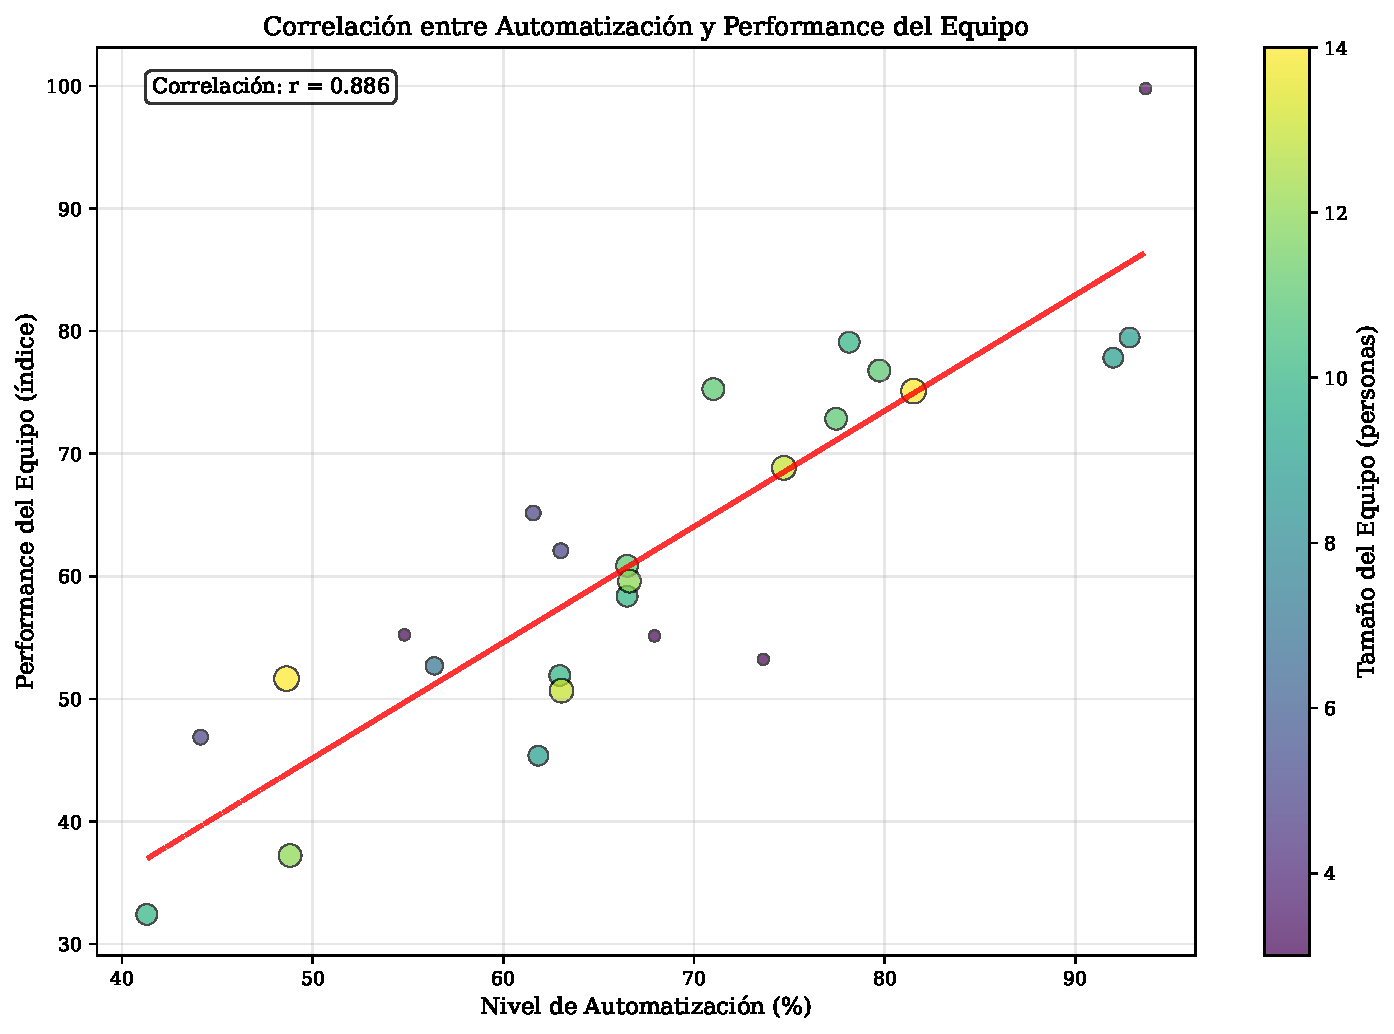
\includegraphics[width=0.46\textwidth]{graphics/correlacion_devops.pdf}
    \caption{Correlación entre nivel de automatización y performance del equipo de desarrollo}
    \label{fig:correlacion_devops}
\end{figure}

La arquitectura backend se fundamenta en Clean Architecture, dividida en capas claramente definidas: Dominio, Aplicación, Infraestructura y Presentación. Esta separación permite una alta cohesión interna y bajo acoplamiento entre capas, facilitando pruebas unitarias y futuras modificaciones. El frontend móvil, desarrollado en Ionic con Angular, adopta una arquitectura de componentes modulares que promueve la reutilización y mantenibilidad.

\subsection{Integración de Tecnologías Emergentes}

Codexy incorpora tecnologías emergentes que amplían su capacidad:

- **Inteligencia Artificial**: Integración con Azure Cognitive Services para reconocimiento de imágenes en códigos QR dañados.

- **Internet de las Cosas (IoT)**: Compatibilidad con sensores RFID para inventarios automatizados en almacenes inteligentes.

- **Blockchain**: Opcional para trazabilidad inmutable de movimientos de inventario en contextos regulatorios estrictos.

- **Realidad Aumentada**: Soporte para visualización AR de ubicaciones de items en bodegas.

\subsection{Optimización de Rendimiento}

Implementamos varias estrategias de optimización:

- **Caching**: Uso de Redis para datos frecuentemente accedidos, reduciendo latencia de base de datos.

- **Compresión**: GZIP para respuestas API, reduciendo ancho de banda en un 60\%.

- **Lazy Loading**: Carga diferida de módulos en la aplicación móvil para tiempos de inicio más rápidos.

- **CDN**: Distribución de assets estáticos mediante Azure CDN para carga global optimizada.

\subsection{Pipelines de Integración Continua}

Implementamos pipelines de CI/CD utilizando GitHub Actions, automatizando procesos desde el commit hasta el despliegue. Cada push a ramas principales activa:

1. Análisis estático de código con SonarQube para detectar vulnerabilidades y deuda técnica.

2. Ejecución de suites de pruebas unitarias y de integración con cobertura mínima del 80\%.

3. Construcción de imágenes Docker para entornos consistentes.

4. Despliegue automático a entornos de staging y producción mediante estrategias de blue-green deployment.

Esta automatización reduce el tiempo de feedback y minimiza errores de despliegue, permitiendo releases frecuentes y confiables.

\subsection{Prácticas de Desarrollo y Calidad}

Aplicamos rigurosas prácticas de calidad de código:

- **Formateo y Linting**: Utilizamos Prettier para JavaScript/TypeScript y C\# Analyzer para .NET, asegurando consistencia en el estilo de código.

- **Pruebas Automatizadas**: Implementamos pirámide de pruebas con énfasis en unitarias (xUnit para backend, Jasmine/Karma para frontend), integradas (usando TestServer en .NET) y end-to-end con Cypress.

- **Análisis Estático de Seguridad (SAST)**: Herramientas como Checkmarx y OWASP ZAP escanean el código en busca de vulnerabilidades comunes como inyección SQL o XSS.

- **Monitoreo**: Integración con Application Insights para telemetría en tiempo real, alertas proactivas y análisis de rendimiento.

Estas prácticas no solo elevan la calidad del software, sino que también aceleran el desarrollo al detectar problemas temprano en el ciclo.

\subsection{Fragmento de código}

A continuación, presentamos un ejemplo de implementación de una función con tipado estático en el backend de Codexy, ilustrando el uso de Clean Architecture:

\ifminted
\begin{minted}[linenos]{csharp}
// Capa de Dominio
public class Item
{
    public Guid Id { get; private set; }
    public string Name { get; private set; }
    public string QrCode { get; private set; }

    public Item(string name, string qrCode)
    {
        Id = Guid.NewGuid();
        Name = name ?? throw new ArgumentNullException(nameof(name));
        QrCode = qrCode ?? throw new ArgumentNullException(nameof(qrCode));
    }
}

// Capa de Aplicación
public interface IItemService
{
    Task<ItemDto> GetItemByQrCodeAsync(string qrCode);
}

public class ItemService : IItemService
{
    private readonly IItemRepository _itemRepository;

    public ItemService(IItemRepository itemRepository)
    {
        _itemRepository = itemRepository;
    }

    public async Task<ItemDto> GetItemByQrCodeAsync(string qrCode)
    {
        var item = await _itemRepository.GetByQrCodeAsync(qrCode);
        return item != null ? new ItemDto { Id = item.Id, Name = item.Name } : null;
    }
}
\end{minted}
\else
\begin{lstlisting}[language=C#]
// Capa de Dominio
public class Item
{
    public Guid Id { get; private set; }
    public string Name { get; private set; }
    public string QrCode { get; private set; }

    public Item(string name, string qrCode)
    {
        Id = Guid.NewGuid();
        Name = name ?? throw new ArgumentNullException(nameof(name));
        QrCode = qrCode ?? throw new ArgumentNullException(nameof(qrCode));
    }
}

// Capa de Aplicación
public interface IItemService
{
    Task<ItemDto> GetItemByQrCodeAsync(string qrCode);
}

public class ItemService : IItemService
{
    private readonly IItemRepository _itemRepository;

    public ItemService(IItemRepository itemRepository)
    {
        _itemRepository = itemRepository;
    }

    public async Task<ItemDto> GetItemByQrCodeAsync(string qrCode)
    {
        var item = await _itemRepository.GetByQrCodeAsync(qrCode);
        return item != null ? new ItemDto { Id = item.Id, Name = item.Name } : null;
    }
}
\end{lstlisting}
\fi

Este fragmento demuestra la separación de responsabilidades, inyección de dependencias y uso de interfaces para facilitar pruebas.

\subsection{Comparación de tecnologías}

La selección de tecnologías se basó en criterios objetivos como madurez, comunidad, rendimiento y alineación con los requerimientos del proyecto. La \cref{tab:frameworks} presenta una comparación detallada de los frameworks evaluados, destacando por qué .NET 9 e Ionic fueron seleccionados sobre alternativas como Node.js puro o React Native.

\input{tables/frameworks_comparison.tex}

En resumen, la implementación de Codexy combina tecnologías modernas con prácticas de ingeniería de software sólidas, resultando en un sistema robusto, escalable y mantenible que satisface las necesidades de gestión de inventarios en entornos institucionales complejos.

\subsection{Despliegue y Escalabilidad}

Para el despliegue, utilizamos contenedores Docker para garantizar consistencia entre entornos de desarrollo, staging y producción. La orquestación se maneja con Kubernetes, permitiendo escalado automático basado en métricas de CPU y memoria. Implementamos estrategias de blue-green deployment para minimizar downtime durante actualizaciones, y utilizamos Azure Application Insights para monitoreo en tiempo real y alertas proactivas.

La arquitectura soporta escalabilidad horizontal mediante la adición de nodos, y vertical mediante la optimización de consultas a base de datos con índices apropiados y técnicas de caching con Redis. Para la resiliencia, implementamos circuit breakers y retry policies para manejar fallos temporales en servicios externos.

\subsection{Seguridad y Cumplimiento}

Más allá de JWT, implementamos OAuth 2.0 para integración con sistemas de identidad corporativos, y encriptación end-to-end para datos sensibles. Cumplimos con estándares como GDPR para protección de datos personales y SOX para controles internos en instituciones educativas. Realizamos penetration testing trimestral y auditorías de seguridad externa para mantener la confianza de los usuarios.